% Informe de Trabajo de Título - Fabián Ortega Llantén
% Formato según Reglamento TT vf2024: carta, márgenes 2,5 cm, Times 12,
% párrafos justificados con sangría 1,27 cm, numeración esquina superior derecha
% desde la portada, citas APA. Cuerpo objetivo: 15 a 25 páginas.
\documentclass[12pt,letterpaper]{article}
\usepackage[utf8]{inputenc}
\usepackage[T1]{fontenc}
\usepackage[spanish,es-tabla]{babel}
\usepackage{newtxtext,newtxmath} % Times
\usepackage[letterpaper,margin=2.5cm]{geometry}
\usepackage{setspace}
\setstretch{1.15}
\usepackage{parskip}
\setlength{\parindent}{1.27cm}
\setlength{\parskip}{6pt}
\usepackage{graphicx}
\usepackage{tikz}
\usetikzlibrary{positioning, fit, arrows.meta}
\usepackage{booktabs}
\usepackage{array}
\usepackage{enumitem}
\setlist{itemsep=2pt, topsep=4pt}
\usepackage{fancyhdr}
\pagestyle{fancy}
\fancyhf{}
\fancyhead[R]{\thepage}
\renewcommand{\headrulewidth}{0pt}
\fancypagestyle{plain}{\fancyhf{}\fancyhead[R]{\thepage}\renewcommand{\headrulewidth}{0pt}}
\usepackage[hidelinks]{hyperref}
\usepackage{titlesec}
\titleformat{\section}{\large\bfseries\MakeUppercase}{\thesection.}{0.6em}{}
\titleformat{\subsection}{\normalsize\bfseries}{\thesubsection}{0.6em}{}
\titleformat{\subsubsection}{\normalsize\itshape\bfseries}{\thesubsubsection}{0.6em}{}
\renewcommand{\thesection}{\Roman{section}}
\renewcommand{\thesubsection}{\arabic{section}.\arabic{subsection}}
\renewcommand{\thesubsubsection}{\arabic{section}.\arabic{subsection}.\arabic{subsubsection}}

\begin{document}

% ==================== PORTADA 1 ====================
\thispagestyle{plain}
\begin{center}
{\normalsize Pontificia Universidad Católica de Chile\\
\textbf{Escuela de Ingeniería}}\\[3.5cm]
{\large\bfseries IMPLEMENTACIÓN DE UNA HERRAMIENTA DE HISTORIAL CLÍNICO CON IA PARA LA GESTIÓN EFICIENTE DE PACIENTES EN UNA UNIDAD DE PACIENTE CRÍTICO}\\[2.5cm]
{\large\bfseries Fabián Ignacio Ortega Llantén}\\[2cm]
Trabajo de Título para optar al título de\\
Ingeniero Civil de Industrias, Diploma en Ingeniería en Tecnologías de Información\\[2cm]
Profesor Guía:\\[0.3cm]
{\bfseries Denis Parra Santander}\\[2cm]
Santiago de Chile, 2026
\end{center}
\newpage

% ==================== PORTADA 2 ====================
\begin{center}
{\normalsize Pontificia Universidad Católica de Chile\\
Escuela de Ingeniería\\
Departamento de Ciencia de la Computación}\\[3cm]
{\large\bfseries IMPLEMENTACIÓN DE UNA HERRAMIENTA DE HISTORIAL CLÍNICO CON IA PARA LA GESTIÓN EFICIENTE DE PACIENTES EN UNA UNIDAD DE PACIENTE CRÍTICO}\\[2cm]
{\large\bfseries Fabián Ignacio Ortega Llantén}\\[1.5cm]
Trabajo de Título presentado a la Comisión integrada por los profesores:\\[0.5cm]
{\bfseries Denis Parra Santander}\\[0.2cm]
{\bfseries Marcelo Andia Kohnenkampf}\\[0.2cm]
{\bfseries Javier Pereda Torres}\\[1.5cm]
Para completar las exigencias del título de\\
Ingeniero Civil de Industrias, Diploma en Ingeniería en Tecnologías de Información\\[1.5cm]
Santiago de Chile, 2026
\end{center}
\newpage

% ==================== DEDICATORIA ====================
\vspace*{\fill}
\begin{flushright}
\textit{A mi padre, Fabián.}
\end{flushright}
\vspace*{\fill}
\newpage

% ==================== AGRADECIMIENTOS ====================
\section*{AGRADECIMIENTOS}
\addcontentsline{toc}{section}{AGRADECIMIENTOS}

Agradezco a iHealth y al equipo médico y técnico vinculado a la Unidad de Paciente Crítico por abrir las puertas de un problema real y por la confianza depositada durante todo el desarrollo de este trabajo. Trabajar con datos clínicos verdaderos, con las responsabilidades que eso implica, fue una experiencia formativa que no se consigue en un entorno simulado.

A mi profesor guía, Denis Parra, por su disposición durante el proceso. A mi supervisor Marcelo Andia, por acompañamiento, las discusiones técnicas y clínicas, y por empujar el proyecto hacia resultados concretos.

A Rafael Kaempfer, por su apoyo pedagógico durante todo este proceso y por la amistad que construimos en el camino: este trabajo de título fue una de las mejores épocas que he tenido en la universidad, y en buena parte fue gracias a eso.

Al equipo de anotadores clínicos que participó del proceso de construcción del conjunto de referencia, por su rigor y su paciencia con una herramienta que evolucionaba semana a semana con su retroalimentación.

A mi madre, Yohana, y a mis abuelos, Carmen y David, por su apoyo incondicional en cada etapa de este camino y por todo lo que hicieron para que yo pudiera estudiar tranquilo.

Y a mis compañeros más fieles: Kobach, Gastón, Jerson y Toffy, los animales que me hicieron compañía durante todo este proceso. En especial a Toffy, que estuvo a mi lado desde que intenté entrar a la universidad por primera vez, acompañándome incontables horas de estudio apegado a mis pies.
\newpage

% ==================== ÍNDICES ====================
\tableofcontents
\newpage
\listoftables
\listoffigures
\newpage

% ==================== RESUMEN ====================
\section*{RESUMEN}
\addcontentsline{toc}{section}{RESUMEN}

Este trabajo de título se desarrolló en colaboración con iHealth y la Unidad de Paciente Crítico (UPC) del Hospital Dr. Sótero del Río, y abordó un problema estructural de la gestión clínica en unidades de cuidados intensivos: la información más valiosa de cada paciente queda registrada como texto libre en las epicrisis, lo que impide construir estadísticas, auditar decisiones terapéuticas o entrenar modelos predictivos sobre esos datos.

El objetivo del proyecto fue implementar un sistema de software clínico que integre modelos de lenguaje para la extracción automatizada de información desde registros médicos de pacientes de UCI, y evaluar su desempeño frente a un conjunto de referencia anotado por humanos. El trabajo se organizó en torno a dos frentes complementarios: la construcción de una plataforma web de anotación clínica que permite a un equipo de anotadores generar un conjunto de referencia (\textit{ground truth}) confiable a partir de las epicrisis, y la evaluación de modelos de lenguaje de código abierto que intentan extraer automáticamente esas mismas variables.

Sobre el primer frente, se construyó una plataforma completa: ingesta de documentos PDF hacia una base de datos, un mecanismo de anonimización que oculta la identidad del paciente antes de mostrar el documento, un formulario jerárquico de nueve bloques con 199 variables clínicas, un visor seguro que muestra la epicrisis sin entregar el archivo original, y un experimento de concordancia entre anotadores sobre 50 epicrisis con un equipo de anotadores clínicos (cinco en el diseño inicial, ampliado a seis durante la ejecución) y tres revisores por caso.

Sobre el segundo frente, se montó en el clúster de cómputo de iHealth la evaluación de tres modelos de lenguaje abiertos (Gemma, Llama-70B y Qwen) en la extracción de variables clínicas con la evidencia textual que las respalda. Las corridas exploratorias mostraron que, con Gemma, la consulta única del formulario era frágil, y llevaron a un procedimiento de extracción por dominios clínicos (\textit{harness}), sin truncamientos en su validación sobre 5 epicrisis. Como esa mejora no podía atribuirse solo a la división del formulario, se diseñó una comparación controlada sobre las 50 epicrisis del experimento de concordancia y las 199 variables del formulario; su piloto, entre la consulta única y el \textit{harness}, motivó una tercera estrategia, el \textit{harness} con un modelo del caso compartido. La corrida definitiva de las tres estrategias y el acuerdo con la referencia humana están pendientes.

El proyecto exigió, además, resolver problemas propios de un sistema en producción: protección de datos personales sobre 275 epicrisis reales, validación de la migración de la base de datos a un servicio administrado en la nube, respaldos verificados y monitoreo de disponibilidad. El desarrollo permitió evidenciar las tres competencias del perfil de egreso declaradas: el desarrollo de soluciones innovadoras basadas en conocimientos avanzados de Ingeniería de Computación, la aplicación de diversos métodos de análisis de datos, y la investigación y adopción de nuevas tecnologías de información dentro de una organización de salud.
\newpage

% ==================== ABSTRACT ====================
\section*{ABSTRACT}
\addcontentsline{toc}{section}{ABSTRACT}

This thesis was developed in collaboration with iHealth and the Critical Care Unit of Hospital Dr.\ Sótero del Río, addressing a structural problem in intensive care management: the most valuable patient information is recorded as free text in discharge summaries (epicrises), which prevents building statistics, auditing therapeutic decisions, or training predictive models on that data.

The goal of the project was to implement a clinical software system integrating language models for the automated extraction of information from medical records of ICU patients, and to evaluate its performance against a human-annotated reference set. The work was organized around two complementary fronts: building a web-based clinical annotation platform that allows a team of annotators to produce a reliable ground truth from the epicrises, and evaluating open-source large language models that attempt to extract those same variables automatically.

On the first front, a complete platform was built: PDF ingestion into a database, an anonymization mechanism that hides patient identity before displaying each document, a hierarchical annotation form of nine blocks covering 199 clinical variables, a secure viewer that renders the epicrisis without delivering the original file, and an inter-annotator agreement experiment over 50 epicrises with a team of clinical annotators (five in the initial design, expanded to six during execution) and three reviewers per case.

On the second front, an evaluation of three open language models (Gemma, Llama-70B, and Qwen) was set up on the iHealth computing cluster to extract clinical variables together with their supporting textual evidence. Exploratory runs showed that, with Gemma, a single query of the form was fragile, which led to a domain-based extraction procedure (harness) with no truncated outputs in its validation on 5 epicrises. Since that improvement could not be attributed to splitting the form alone, a controlled comparison was designed over the 50 epicrises of the agreement experiment and the form's 199 variables; its pilot, between the single query and the harness, motivated a third strategy, a harness with a shared case model. The definitive run of the three strategies and the agreement with the human reference are pending.

The project also required solving problems inherent to a production system: personal data protection over 275 real epicrises, a validated migration path to a managed cloud database service, verified backups, and availability monitoring. The work provided evidence for the three declared graduate profile competencies: developing innovative solutions based on advanced Computer Science engineering knowledge, applying diverse data analysis methods, and researching and facilitating the adoption of new information technologies within a healthcare organization.
\newpage

% ==================== I. INTRODUCCIÓN ====================
\section{Introducción}

El presente informe describe el trabajo de título desarrollado por el estudiante de Ingeniería Civil de Industrias, Diploma en Ingeniería en Tecnologías de Información, de la Pontificia Universidad Católica de Chile, realizado entre mayo y septiembre de 2026 en colaboración con iHealth y la Unidad de Paciente Crítico del Hospital Dr.\ Sótero del Río. El documento presenta el contexto del proyecto, las actividades desempeñadas, los resultados obtenidos y la forma en que el trabajo evidencia las competencias del perfil de egreso declaradas en la inscripción.

\subsection{Contexto institucional}

\subsubsection{iHealth y la Unidad de Paciente Crítico}

iHealth es un instituto de investigación que reúne a médicos, ingenieros y científicos de datos con el propósito de llevar herramientas de inteligencia artificial a la práctica clínica chilena. El proyecto en que se enmarca este trabajo nace de una necesidad concreta de la Unidad de Paciente Crítico (UPC) del Hospital Dr.\ Sótero del Río: estudiar las comorbilidades de sus pacientes críticos, una pregunta clínica que depende de datos estructurados que hoy no existen, porque la información relevante está dispersa en registros narrativos. A nivel exploratorio, tanto este trabajo como la publicación académica asociada buscan evaluar si modelos de lenguaje (LLM) pueden extraer esa información clínica de forma confiable desde texto narrativo, en el contexto específico de la práctica chilena.

La epicrisis, el resumen médico que se redacta al alta de cada paciente, concentra los antecedentes, el curso clínico, las infecciones, los soportes vitales y los diagnósticos del episodio. Es un documento riquísimo en información y a la vez inutilizable para el análisis sistemático, porque cada médico lo redacta a su manera, en texto libre. Convertir ese texto en datos estructurados y confiables es la condición previa para cualquier análisis estadístico o modelo predictivo sobre la población de la UPC.

\subsubsection{Rol del estudiante}

El estudiante se integró al equipo como responsable del desarrollo de software del proyecto, con un doble mandato: construir la plataforma de anotación clínica con que el equipo médico genera el conjunto de referencia, y montar sobre el clúster de cómputo de iHealth la evaluación de modelos de lenguaje que intentan extraer la misma información de forma automática. El rol incluyó el ciclo completo de un sistema en producción: diseño, implementación, protección de datos personales, infraestructura, operación y soporte a los usuarios clínicos, bajo la supervisión de Marcelo Andia y Rafael Kaempfer por parte de iHealth y la guía académica del profesor Denis Parra.

Este informe describe exclusivamente el trabajo realizado por el estudiante: la plataforma de anotación, el procedimiento de extracción por dominios (\textit{harness}), el protocolo de comparación de estrategias de extracción y la evaluación experimental de los tres modelos de lenguaje en el clúster. Los análisis orientados a publicación científica desarrollados por otros integrantes del equipo quedan fuera del alcance de este documento.

\subsection{Trabajo de título}

\subsubsection{Objetivo general}

Implementar un sistema de software clínico que integre modelos de lenguaje para la extracción automatizada de información desde registros médicos de pacientes en Unidades de Cuidados Intensivos, y evaluar su desempeño mediante coeficientes de concordancia frente a un conjunto de referencia anotado por humanos.

\subsubsection{Objetivos específicos}

\begin{enumerate}
    \item Desarrollar una herramienta de anotación clínica para generar el conjunto de referencia (\textit{ground truth}), capaz de reconstruir la estructura visual de los documentos PDF de origen, con roles diferenciados de administrador y anotador, respaldada por una base de datos consultable y una interfaz web segura para el equipo de anotadores.
    \item Proteger la identidad de los pacientes mediante un mecanismo de anonimización, y operar la plataforma de forma confiable en producción, con monitoreo y respaldos verificados.
    \item Seleccionar y evaluar modelos de lenguaje de código abierto en su capacidad de extraer variables clínicas desde epicrisis reales, exigiendo evidencia textual verificable para cada valor extraído.
    \item Diseñar e implementar un procedimiento de extracción por grupos de variables clínicas (\textit{harness}), con validación de respuestas y una variante con representación compartida del caso, y comparar ambas estrategias con la extracción en una única llamada, sobre los mismos casos y dentro de cada modelo, en términos de validez estructural, fidelidad de la evidencia, coherencia clínica y costo computacional.
    \item Medir la confiabilidad del conjunto de referencia mediante un experimento de concordancia entre anotadores, y comparar el desempeño de los modelos de lenguaje contra ese estándar de referencia humano (comparación programada para completarse antes de la versión final de este informe, una vez que el conjunto de referencia alcance la cobertura suficiente).
\end{enumerate}

\subsubsection{Metodología}

El proyecto se organizó en tres áreas de desarrollo consecutivas y superpuestas. La primera correspondió a la plataforma de anotación clínica: su base de datos, el formulario jerárquico y el visor seguro de documentos. La segunda, a la protección de datos y la infraestructura de producción: el mecanismo de anonimización, la validación de la migración a un servicio administrado en la nube, y el monitoreo y los respaldos verificados. La tercera, a la extracción automática con modelos de lenguaje sobre el clúster de cómputo ih-condor, incluyendo el diseño de un procedimiento de extracción por dominios clínicos y de un protocolo de comparación controlada de tres estrategias de extracción, con el que se contrastará el desempeño de los modelos contra el estándar de referencia humano.

El trabajo siguió un ciclo iterativo con retroalimentación semanal del equipo clínico: cada versión de la plataforma fue usada por anotadores reales, y sus observaciones alimentaron la siguiente iteración. Los requisitos se registraron como historias de usuario en un repositorio de documentación centralizado, y todo el desarrollo quedó versionado en repositorios Git, lo que permite trazar cada afirmación de este informe a trabajo verificable.

\subsubsection{Resultados esperados}

Un sistema integral funcional que permita la extracción de texto clínico, la construcción de un conjunto de referencia confiable con medidas de concordancia entre anotadores, y la evaluación rigurosa de modelos de lenguaje ajustados a las necesidades reales de gestión de pacientes críticos.

En términos verificables, ese resultado se concreta en tres grupos de productos, uno por cada competencia del Capítulo IV: la plataforma de anotación en producción y un protocolo de extracción con un validador común a tres estrategias; la concordancia del conjunto de referencia medida por criterio y una comparación pareada de esas estrategias sobre las 50 epicrisis del experimento de concordancia; y la adopción de estas tecnologías en la organización, con modelos abiertos en el clúster de iHealth sobre un entorno documentado, y con un manual interactivo y un glosario de la plataforma para el equipo clínico.

\subsubsection{Competencias del perfil de egreso}

En la inscripción del trabajo se declararon tres competencias técnicas del perfil de egreso, que se desarrollan en detalle en el Capítulo IV:

\begin{enumerate}
    \item Desarrollar soluciones innovadoras basadas en conocimientos avanzados de Ingeniería de Computación.
    \item Aplicar diversos métodos de análisis de datos para la comprensión de los fenómenos abordados.
    \item Investigar sobre nuevas tecnologías de información existentes en la industria y facilitar su adopción dentro de las organizaciones.
\end{enumerate}

% ==================== II. ACTIVIDADES ====================
\section{Actividades desempeñadas}

Este capítulo describe el trabajo realizado, organizado por líneas de desarrollo. La dedicación total registrada en las bitácoras del período fue de 573 horas, distribuidas entre mayo y septiembre de 2026.

\subsection{Conceptualización y análisis exploratorio}

El proyecto comenzó con una reunión de definición junto al equipo médico y técnico de iHealth, en la que se acordó el problema central a nivel exploratorio (evaluar la extracción de información clínica desde texto narrativo mediante modelos de lenguaje, con foco en las comorbilidades de pacientes críticos, en el contexto de la práctica chilena) y una visión dual: generar publicaciones académicas y, a la vez, un producto funcional integrable en sistemas hospitalarios. Se exploraron 27 epicrisis reales de la UPC, aplicando anonimización manual y automática para proteger la información sensible de los pacientes, y se ejecutó un análisis de agrupamiento (\textit{clustering}) de comorbilidades que permitió identificar perfiles de paciente y validar la viabilidad de extraer información estructurada desde texto clínico no estructurado.

En paralelo, el estudiante completó un proceso de formación técnica autodidacta de diez capítulos, que abarcó fundamentos matemáticos, aprendizaje de máquina, redes neuronales, procesamiento de lenguaje natural, \textit{embeddings}, mecanismos de atención, arquitecturas Transformer (Vaswani et al., 2017), modelos de lenguaje (GPT/LLM) con implementación práctica en PyTorch, modelos de supervivencia e inteligencia artificial aplicada a medicina, junto con la configuración del acceso al clúster de cómputo de iHealth (ih-condor): autenticación, desarrollo remoto y buenas prácticas de almacenamiento en un entorno compartido.

\subsection{Plataforma de anotación clínica}

La pieza central del primer frente fue una plataforma web donde los anotadores clínicos registran, para cada epicrisis, el valor de un conjunto de variables definidas junto al equipo médico.

\subsubsection{Ingesta y base de datos}

Se desarrolló el flujo de ingesta de los documentos PDF hacia una base de datos PostgreSQL, junto con la interfaz base de anotación, métricas de consistencia entre evaluadores y la guía oficial de anotación. Sobre esa base se iteró durante todo el proyecto: migración a escrituras atómicas para manejar concurrencia, validaciones de fechas, pruebas unitarias y de extremo a extremo, verificación de desviaciones de esquema y un canal de notificaciones para el monitoreo remoto del sistema.

\subsubsection{Formulario jerárquico de anotación}

El formulario se rediseñó en una estructura jerárquica de nueve bloques desplegables con 199 variables finales, pensada para recorrer documentos largos sin saltarse campos. Cada variable booleana admite Sí, No o duda con grado de sospecha; las fechas se capturan en dos pasos; y un buscador con sinónimos y códigos de la clasificación internacional de enfermedades permite ubicar cada variable por el nombre que usó el médico. Iteraciones posteriores incorporaron el inicio en blanco (distinguir un ``No'' decidido de una variable aún no revisada), la propagación de respuestas desde variables madre a sus dependientes, la captura de múltiples evidencias por variable y la corrección de un defecto que borraba trabajo ya anotado al cambiar una sección de estado. Estas decisiones quedaron registradas como historias de usuario y respaldadas por pruebas automatizadas.

\subsubsection{Visor seguro de documentos}

Para que el anotador vea la epicrisis sin que el archivo original llegue a su navegador, se construyó un visor propio: la estructura visual de cada documento (posición, tamaño y fuente de cada bloque de texto) se extrae del PDF y se guarda en la base de datos, y un servicio la entrega solo a quien tiene sesión iniciada, el rol adecuado y el caso asignado. El visor reconstruye cada página en pantalla y permite capturar evidencia con un clic sobre el propio texto; la Figura~\ref{fig:vista-formulario} muestra el formulario jerárquico durante una sesión de revisión en vivo.

\begin{figure}[htbp]
\centering
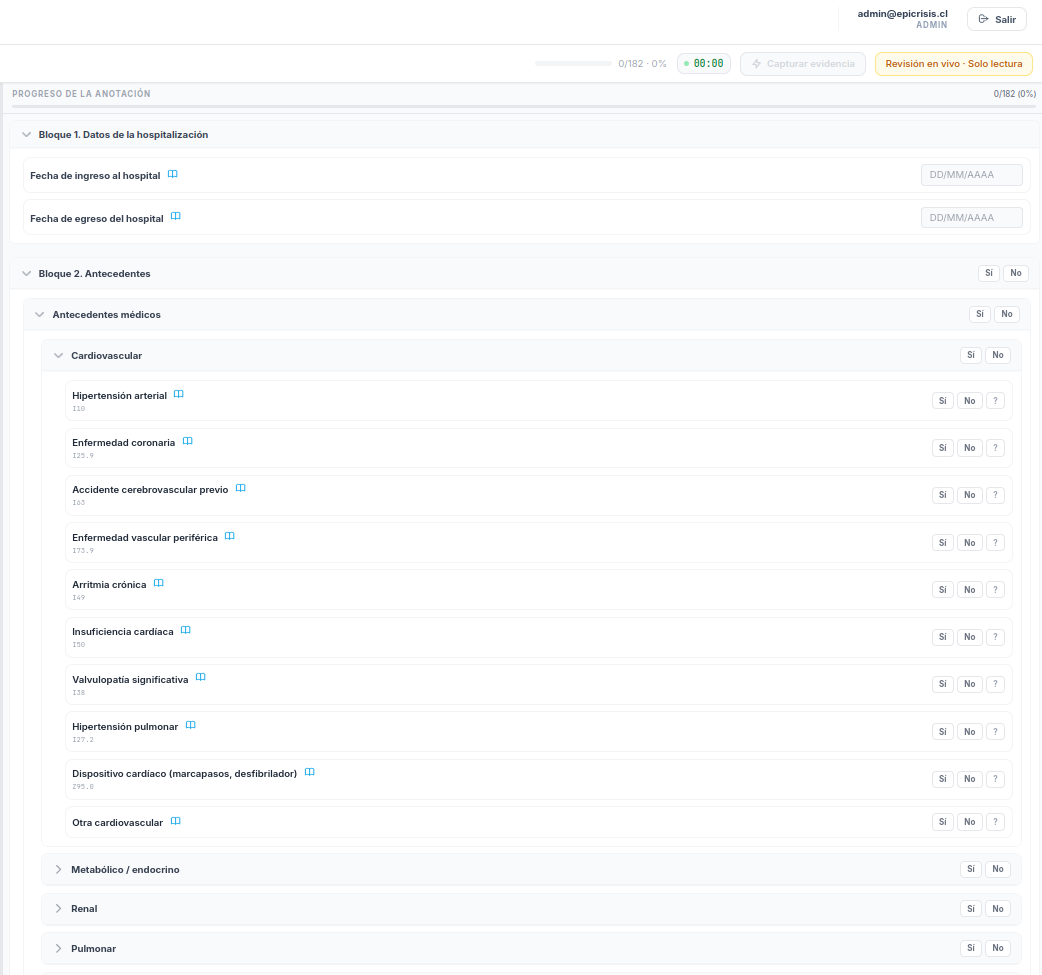
\includegraphics[width=\textwidth]{figuras/capturas/vista_anotacion_formulario.png}
\caption{Formulario jerárquico de anotación con su barra de progreso, en modo de revisión en vivo.}
\label{fig:vista-formulario}
\end{figure}

\subsection{Protección de datos personales}

El trabajo con epicrisis reales exigió un mecanismo de anonimización en constante endurecimiento. La primera versión ocultaba RUT, dirección, nombre y firmas médicas al momento de entregar el documento, usando bloques del mismo largo que el texto tapado para no descuadrar la página. Iteraciones posteriores agregaron teléfono, fecha de nacimiento, comuna, número de archivo y correo electrónico, y corrigieron casos límite detectados en uso real: apellidos que contienen términos médicos, cargos clínicos cuya eliminación mutilaba palabras legítimas (el caso del cargo TENS dentro de ``hipertensión''), y menciones negadas de la terapia HFAV. La reconstrucción final del procedimiento se validó primero sobre 28 documentos y luego sobre los 275 originales, generando la planilla y la base de datos desde una misma fuente, con una entrega cifrada acompañada de inventario, diccionario de datos y huellas de verificación.

Este frente incluyó además la gestión de un incidente real, ocurrido en mayo de 2026: un proceso automatizado sobrescribió la base de datos de producción, dejando expuesta información personal identificable. El estudiante diagnosticó el alcance del problema y respondió con tres correcciones de emergencia en secuencia: primero la anonimización de las 434 ocurrencias afectadas para contener la exposición, luego la reparación del renderizador del frontend que la había provocado, y finalmente una migración idempotente de la base de datos para dejar el esquema en un estado consistente y repetible. Como consecuencia de mediano plazo del incidente, se incorporaron los respaldos verificados y las alertas de frescura que se describen en la sección de infraestructura, de modo que un problema similar se detecte automáticamente en vez de descubrirse por inspección manual.

\subsection{Evaluación de modelos de lenguaje en el clúster}

El segundo frente evaluó si un modelo de lenguaje de código abierto puede extraer por sí solo las variables que los anotadores marcan a mano. Se optó por modelos de código abierto, descartando servicios propietarios por API, porque el requisito de no sacar información clínica identificable fuera del entorno controlado de iHealth exigía correr la inferencia íntegramente dentro del clúster ih-condor; dentro de esa restricción se seleccionaron Gemma, Llama-70B (Grattafiori et al., 2024) y Qwen. Sobre el clúster ih-condor se configuró primero una corrida mínima con el modelo Gemma, sin aleatoriedad, apuntando a los 48 campos iniciales del formulario y exigiendo que cada valor venga acompañado del fragmento de texto que lo respalda. Superada esa prueba de circuito completo, se ejecutó una evaluación exploratoria de los tres modelos sobre una cohorte de 20 casos, con una consulta única de esos mismos 48 campos. Cada ejecución se limitó a tres horas para poder reanudarla, se corrigió la reserva de tarjetas gráficas al detectar que uno de los modelos debía repartirse entre varias, y se versionaron los resultados, el registro de cada consulta y los archivos de ejecución.

A partir de los primeros resultados se rediseñó el procedimiento de consulta: en lugar de una única llamada al modelo, la extracción se dividió en un mapa inicial del caso y cinco consultas especializadas por dominio clínico (antecedentes, episodio en la UCI, infecciones, fallas orgánicas y diagnósticos). Así cada llamada abarca menos, se valida por separado y puede reintentarse sin rehacer todo. Se endureció además la exigencia de evidencia: el modelo ya no redacta la cita, sino que señala qué fragmento numerado de la epicrisis la respalda, y el sistema copia ese tramo literal, eliminando la posibilidad de evidencia inventada.

Como ese rediseño cambió varias condiciones a la vez, la etapa final se dedicó a separar sus efectos con un protocolo de comparación controlada que enfrenta la consulta única con la división del formulario en 18 grupos, sobre las 50 epicrisis del experimento de concordancia; su piloto motivó una tercera estrategia, apoyada en un modelo del caso que retoma el mapa inicial (sección~\ref{sec:estrategias}).

\subsection{Experimento de concordancia entre anotadores}

Para la construcción del estándar de referencia se incorporó un equipo de cinco anotadores clínicos, que al cierre de este informe se encuentran anotando en producción sobre la plataforma. El proceso de incorporación se resolvió dentro de la propia aplicación: en el primer inicio de sesión se exige la aceptación de términos y condiciones, y el anotador dispone de un manual integrado con ejemplos interactivos (un documento clínico simulado y una versión reducida del formulario donde practicar sin afectar casos reales) y un glosario clínico con buscador. El estudiante desarrolló la implementación de estas herramientas dentro de la aplicación, sobre la base del protocolo de anotación y el video tutorial elaborados por otros integrantes del equipo.

La asignación de casos sigue un diseño combinatorio balanceado: 50 epicrisis se distribuyen de modo que cada caso sea revisado por tres anotadores, lo que produce 150 asignaciones y permite estimar la concordancia entre todos los pares mediante kappa de Cohen. En el diseño inicial, con cinco anotadores, cada uno recibía 30 casos y cada pareja compartía exactamente 15; ese reparto parejo cambió durante la ejecución cuando el equipo creció a seis personas (sección~\ref{sec:concordancia}). La selección de los 50 casos es determinista y auditable (un hash con semilla fija sobre el identificador anonimizado de cada paciente), y la asignación se verifica programáticamente antes de aplicarse en una transacción única.

Durante la anotación, la plataforma ofrece supervisión en dos niveles: un panel de administración con la matriz de avance caso por anotador y revisión en vivo (el administrador abre la misma vista de anotación en modo de solo lectura, con actualización automática), y una derivación automática a revisión experta cuando un caso acumula criterios marcados como no determinables. Durante la ejecución, el estudiante acompañó el avance de cada anotador, atendió consultas y corrigió los defectos que el uso intensivo hizo visibles.

\subsection{Infraestructura y operación}

El paso de prototipo a sistema en uso exigió infraestructura seria. Se validó la migración de la base de datos desde un computador local a un servicio administrado en la nube en la región sudamericana, con conexión cifrada y verificación efectiva del certificado del servidor; durante el experimento de concordancia, la base opera localmente, replicada cada hora hacia ese proveedor en la nube.

La operación se supervisa mediante lazos de monitoreo concéntricos que convergen en un mismo canal de mensajería (esquematizados en la Figura~\ref{fig:monitoreo} del Anexo B). En el lazo interno, el supervisor de procesos reinicia automáticamente la API ante cualquier caída. En un segundo nivel, un bot de Telegram que corre como proceso independiente (de modo que sobrevive a una caída de la API y puede levantarla remotamente) emite cuatro reportes diarios que combinan el estado de los servicios, el uso de disco y de registros de transacciones de la base de datos, y el avance del experimento por anotador; el mismo bot notifica en tiempo real los inicios de sesión de los anotadores y sus avances sustanciales, con umbrales y períodos de enfriamiento para evitar ruido. En el nivel más externo, un flujo de integración continua ejecutado fuera de la infraestructura propia verifica cada quince minutos el frontend y el backend mediante una sonda sintética que ejercita la ruta pública, la API y una consulta real a la base de datos, registrando cada corte como un aviso que se abre y cierra automáticamente.

Los respaldos siguen la misma lógica de verificación: la base se replica cada hora hacia un proveedor secundario con comparación de conteos tabla por tabla, complementada por volcados cifrados con verificación de suma de comprobación. Tras detectar que la copia de respaldo llevaba doce días sin actualizarse sin que ninguna alerta lo advirtiera, se sumó un verificador de frescura que alerta si el último respaldo verificado supera las tres horas de antigüedad.

\subsection{Desafíos encontrados}

Tres desafíos marcaron el proyecto. El primero fue trabajar con datos clínicos reales: cada decisión técnica tuvo una dimensión de responsabilidad sobre la privacidad de pacientes verdaderos, y los defectos del anonimizador no eran errores abstractos sino riesgos concretos. El segundo fue diseñar software para usuarios sin formación técnica, en un dominio (la medicina clínica) ajeno a la formación del propio estudiante: el equipo de anotadores está compuesto por profesionales clínicos, no por desarrolladores, y cada fricción de la interfaz se traducía directamente en pérdida de calidad del conjunto de referencia; la retroalimentación semanal con el equipo médico obligó a un ritmo de iteración alto. El tercero fue operar un sistema en producción con recursos acotados: los incidentes de la base de datos y del respaldo silencioso mostraron que la confiabilidad no se declara, se construye con verificación y monitoreo.

% ==================== III. RESULTADOS ====================
\section{Resultados}

\subsection{Plataforma de anotación operativa}

El resultado más visible del proyecto es una plataforma de anotación clínica en producción, usada por un equipo real de anotadores sobre 275 epicrisis anonimizadas de la UPC. La plataforma integra el formulario jerárquico de 199 variables, el visor seguro de documentos, la captura de evidencia textual, el manual interactivo de entrenamiento y un panel de administración con búsqueda, seguimiento del avance por anotador y exportación de resultados.

\subsection{Conjunto de datos protegido y trazable}

Las 275 epicrisis originales fueron procesadas por un procedimiento de anonimización validado iterativamente, con una entrega final cifrada que incluye inventario, diccionario de datos y huellas de verificación. La auditoría de la versión final verificó 1.455 componentes de identidad procesados, con cero RUT, cero teléfonos y cero correos residuales, y sin corrupciones del texto clínico. La base de datos de anotación y la planilla de análisis se generan desde una misma fuente, lo que garantiza consistencia entre lo que ven los anotadores y lo que consumen los análisis posteriores.

\subsection{Evaluación de modelos de lenguaje: infraestructura y etapa exploratoria}

Sobre el clúster ih-condor (8 GPU NVIDIA RTX A6000 de 48~GiB, planificador SLURM) el estudiante montó la infraestructura de evaluación de tres modelos de lenguaje abiertos (Gemma, Llama-70B y Qwen) en la extracción de variables clínicas con evidencia textual verificable: corridas deterministas y reanudables sobre una cohorte exploratoria de 20 casos con los 48 campos iniciales del formulario, con resultados, registro de cada consulta y archivos de ejecución versionados.

El resultado consolidado de esta etapa es metodológico. Las corridas exploratorias mostraron que la consulta única era frágil: con Gemma, las respuestas llegaban truncadas y cada paciente tomaba cerca de media hora. El procedimiento de extracción por dominios clínicos (\textit{harness}) diseñado en respuesta, que además detiene la generación al cerrarse la estructura de datos, se validó con Gemma sobre 5 epicrisis (Tabla~\ref{tab:harness}); con esa misma detención, la consulta única de Gemma tampoco se truncó en una corrida posterior sobre los 20 casos.

\begin{table}[h]
\centering
\begin{tabular}{lc}
\toprule
\textbf{Métrica (validación sobre 5 epicrisis)} & \textbf{Extracción por dominios (\textit{harness})} \\
\midrule
Respuestas con estructura de datos completa & 44 de 44 \\
Truncamientos & 0 \\
Reducción de tiempo por paciente & $\sim$5,5$\times$ \\
\bottomrule
\end{tabular}
\caption{Validación exploratoria del procedimiento por dominios clínicos con Gemma (5 epicrisis, 48 campos iniciales). La reducción de tiempo se mide frente a la primera versión del mismo procedimiento, en las 2 epicrisis que ambas completaron.}
\label{tab:harness}
\end{table}

En esa validación, 2 de las 5 epicrisis terminaron con citas no literales, lo que llevó a pedir al modelo el número del fragmento de respaldo en lugar del texto de la cita. Ese cambio impide por construcción las citas inventadas, pero no que se cite un pasaje insuficiente: en un caso, el procedimiento marcó hemofiltración de alto volumen a partir de un pasaje que solo documentaba hemofiltración continua.

\subsection{Estrategias de extracción: diseño de la comparación y piloto}\label{sec:estrategias}

La validación anterior mostraba una ventaja del \textit{harness}, pero no permitía atribuirla a la división del formulario: el procedimiento nuevo cambió a la vez la forma de pedir las variables y el criterio de detención de la generación, y poco después también la forma de citar la evidencia. Para aislar ese efecto se construyó un protocolo de comparación controlada, versionado y cubierto por pruebas sintéticas, en el que todas las estrategias reciben la misma epicrisis completa con sus líneas numeradas, las mismas reglas del manual de anotación y el mismo formulario de 199 variables, responden con el mismo formato y pasan por el mismo validador de tipos, evidencia, relaciones jerárquicas y exclusiones. Las estrategias difieren solo en cómo se pide el formulario (Figura~\ref{fig:estrategias}). A diferencia de las corridas exploratorias sobre 20 casos, el protocolo usa las 50 epicrisis del experimento de concordancia, de modo que cada respuesta del modelo pueda contrastarse con la anotación humana del mismo paciente.

\begin{itemize}
    \item \textbf{Estrategia A, consulta única:} una sola llamada devuelve las 199 variables.
    \item \textbf{Estrategia B, \textit{harness}:} 18 llamadas independientes, cada una con un grupo de hasta 16 variables de un mismo bloque del formulario, que se validan y reintentan por separado y luego se unen.
    \item \textbf{Estrategia C, \textit{harness} con modelo del caso compartido:} una llamada previa construye un modelo estructurado del episodio (estadías en UCI, línea de tiempo, problemas clasificados como antecedente o evento agudo, soportes, infecciones y desenlace) en el que cada afirmación cita las líneas de la epicrisis que la respaldan. Ese modelo se valida como cualquier otra salida y se entrega a las mismas 18 llamadas de la estrategia B.
\end{itemize}

\begin{figure}[htbp]
\centering
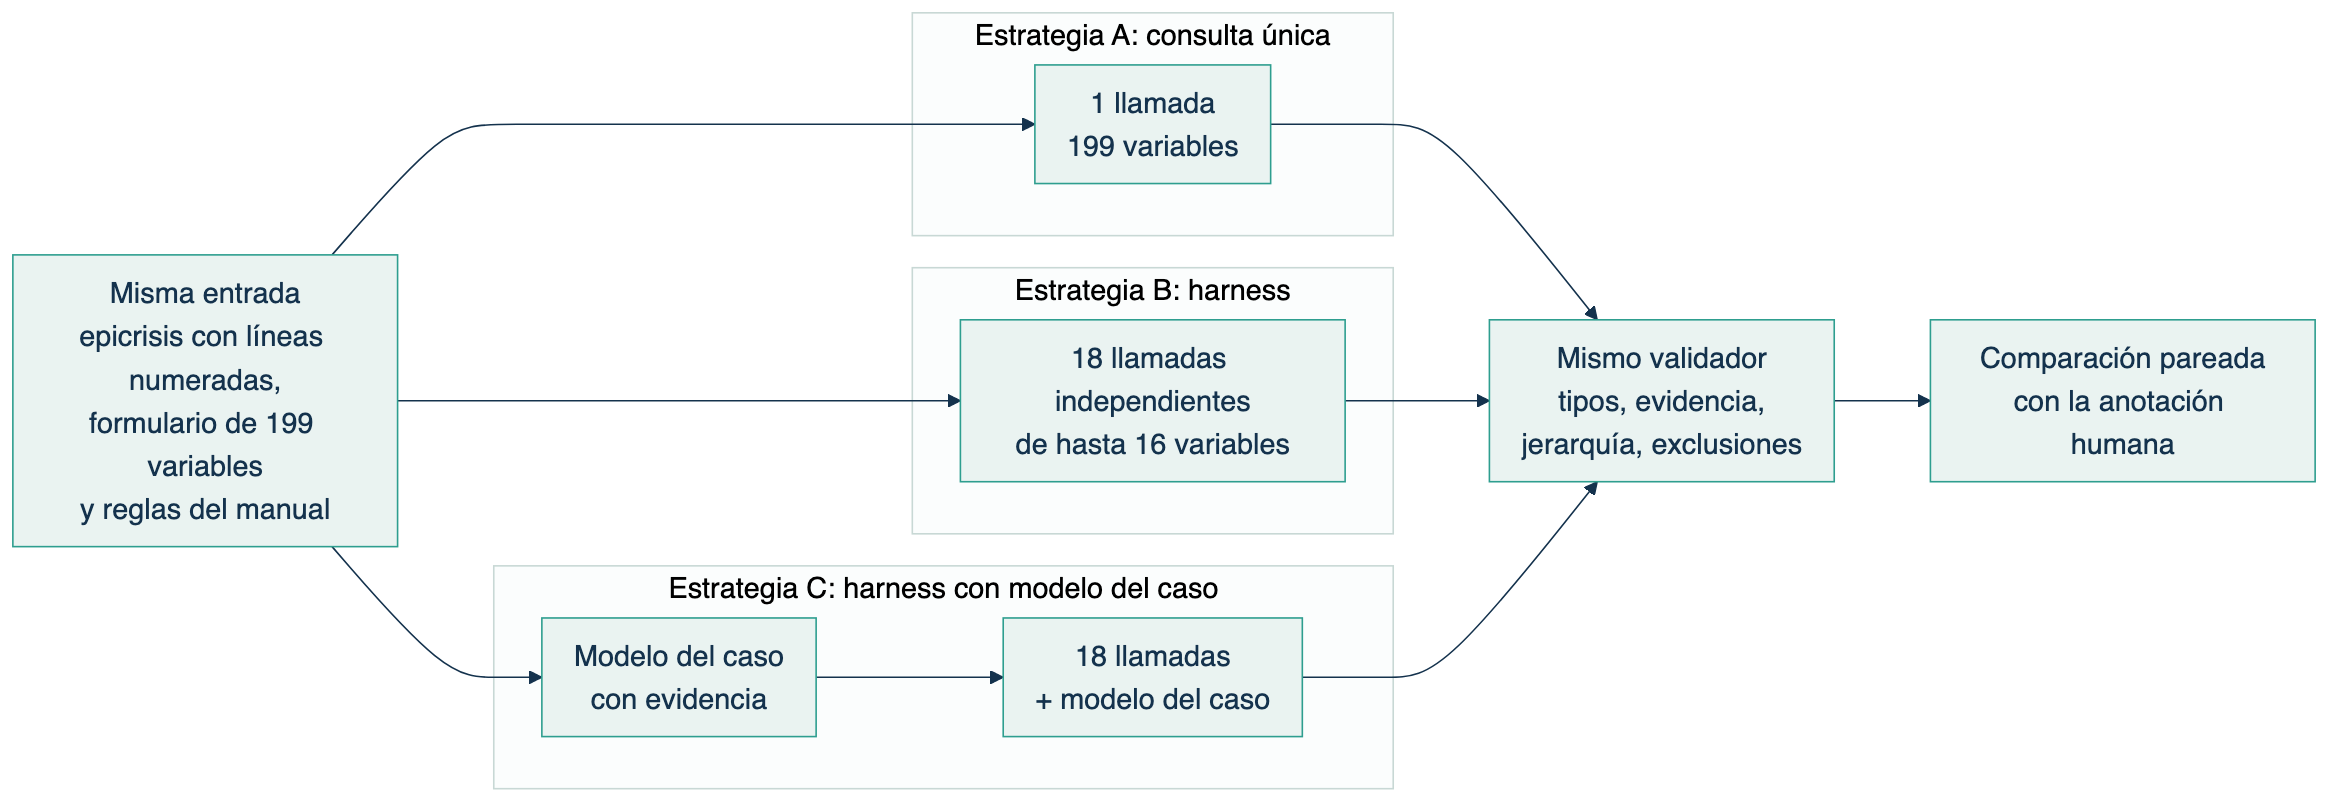
\includegraphics[width=\textwidth]{figuras/diagramas/fig_estrategias.png}
\caption{Las tres estrategias de extracción comparadas. Comparten la entrada, el formulario, las reglas y el validador, y difieren solo en cómo se pide el formulario; la estrategia C agrega una llamada previa que construye un modelo del caso compartido por sus 18 llamadas.}
\label{fig:estrategias}
\end{figure}

En la estrategia C la epicrisis prevalece sobre el modelo del caso: la evidencia de cada variable debe citar líneas de la nota, y si el modelo del caso no supera la validación, el caso se registra como fallido en lugar de completarse con la estrategia B. La comparación principal, definida antes de contrastar cualquier salida con la referencia humana, es la no inferioridad de la estrategia B frente a la A en el acuerdo con los anotadores; las comparaciones de la estrategia C con la A y con la B son secundarias. Además del acuerdo se miden la validez estructural, la fidelidad de la evidencia, el costo (llamadas, tokens y tiempo) y la coherencia clínica entre bloques del formulario, mediante reglas que se definirán con el equipo clínico (por ejemplo, sepsis sin infección registrada o fechas de ventilación sin ventilación).

Antes de la corrida definitiva se ejecutó un piloto de las estrategias A y B con Gemma sobre una epicrisis de la cohorte (Tabla~\ref{tab:piloto}). Al revisarla, el caso resultó ser una hospitalización quirúrgica electiva sin estadía en UCI, por lo que el piloto verifica el funcionamiento del procedimiento, no la extracción de variables de UCI, y no permite concluir sobre la calidad de ninguna estrategia.

\begin{table}[htbp]
\centering
\begin{tabular}{lcc}
\toprule
\textbf{Métrica (piloto, 1 epicrisis)} & \textbf{A: consulta única} & \textbf{B: \textit{harness}} \\
\midrule
Variables con respuesta válida & 199 de 199 & 199 de 199 \\
Llamadas (reintentos) & 2 (1) & 20 (2) \\
Unidades válidas al primer intento & 0 de 1 & 16 de 18 \\
Respuestas truncadas & 0 & 0 \\
Caso válido tras los reintentos & Sí & No (6 errores de relación) \\
Tokens generados & 25.485 & 14.831 \\
Tiempo total & 3 h 47 min & 39 min \\
Memoria máxima de GPU (suma de las dos) & 50,2 GB & 22,1 GB \\
Evidencias con texto idéntico a la nota & 14 de 14 & 10 de 10 \\
\bottomrule
\end{tabular}
\caption{Piloto de las estrategias A y B con Gemma, cuantizado a 4 bits en dos GPU RTX A6000, sobre una epicrisis sin estadía en UCI. Verifica el procedimiento; no tiene valor inferencial.}
\label{tab:piloto}
\end{table}

El piloto dejó tres observaciones. La primera es de costo: ambas estrategias entregaron las 199 variables sin truncamiento y con evidencia cuyo texto coincide con la nota, pero la consulta única tuvo que generar cerca de 12.700 tokens en una sola respuesta y, al fallar la validación de su primer intento, rehacer el formulario completo, lo que la llevó a 3 h 47 min frente a los 39 min del \textit{harness}. La segunda es un modo de falla propio de la división: el grupo que registra las fechas de ventilación mecánica invasiva no disponía de la respuesta de otro grupo, que había indicado que no hubo ventilación, y dejó esas fechas como no documentadas en lugar de no aplicables, lo que produjo 6 violaciones de relaciones jerárquicas. Ese error, propio de llamadas que no ven las respuestas de las demás, motivó la estrategia C. La tercera es de reproducibilidad: las versiones sucesivas del protocolo produjeron respuestas idénticas en las 20 llamadas del \textit{harness}, lo que indica que la inferencia sin aleatoriedad es repetible en el clúster.

La corrida definitiva, con las 50 epicrisis, las tres estrategias y los tres modelos, con la tabla de comportamiento de inferencia (latencia, velocidad de generación, memoria y truncamientos) y las métricas de acuerdo contra el estándar de referencia humano, se ejecutará una vez cerrado el experimento de concordancia. La estrategia C está implementada y su piloto se encuentra en curso; los resultados se incorporarán en la versión final de este informe.

\subsection{Experimento de concordancia en ejecución}\label{sec:concordancia}

El experimento de concordancia entre anotadores quedó diseñado, instrumentado y en ejecución: 50 epicrisis, un equipo de anotadores (cinco en el diseño inicial, seis desde el rebalanceo descrito más abajo), tres revisores por caso, 150 asignaciones, con selección reproducible de casos y una vista de administración que calcula la concordancia sin interferir con el trabajo de anotación.

El experimento avanza a ritmo sostenido: al corte del 27 de agosto de 2026 registraba 23 de las 150 asignaciones entregadas, y al corte verificado del 7 de septiembre alcanzó 58, con 27 casos con una anotación completa, 14 con dos, 1 con las tres y 8 aún sin entregas. Durante ese período se rebalanceó además la carga entre los revisores médicos del equipo: el oncólogo del equipo, sin avance registrado, traspasó 15 de sus 30 asignaciones al supervisor clínico del proyecto mediante una transacción única, incorporándolo como sexto revisor. El diseño se mantuvo intacto donde importa para la concordancia (150 asignaciones, tres revisores por caso), aunque el reparto ya no es parejo entre las seis personas que participan.

Al corte del 15 de septiembre de 2026, con 43 epicrisis que cuentan con dos o más anotaciones enviadas y 222 criterios evaluados, la concordancia inter-anotador preliminar alcanza un kappa de Cohen promedio de 0,72, calculado por pares de anotadores y por criterio sobre las frecuencias marginales observadas, un acuerdo sustancial en la escala de Landis y Koch (1977) (Figura~\ref{fig:irr}). La distribución por criterio muestra la heterogeneidad esperable: 158 de los 222 criterios (71\%) alcanzan acuerdo sustancial (kappa sobre 0,6), 21 quedan en rango moderado y 43 (19\%) bajo 0,4. Dentro de este último grupo, 30 criterios exhiben kappa nulo o negativo pese a acuerdos porcentuales iguales o superiores al 82\%, la conocida paradoja del kappa en categorías de prevalencia extrema; 7 de esos 30 corresponden a categorías residuales del formulario (los campos de tipo ``otra''). El desacuerdo genuino se concentra en la identificación del foco respiratorio de infección (47\% de acuerdo), un hallazgo accionable para la siguiente revisión de la guía de anotación. Los valores definitivos, con el experimento cerrado, se reportarán en la versión final.

\begin{figure}[htbp]
\centering
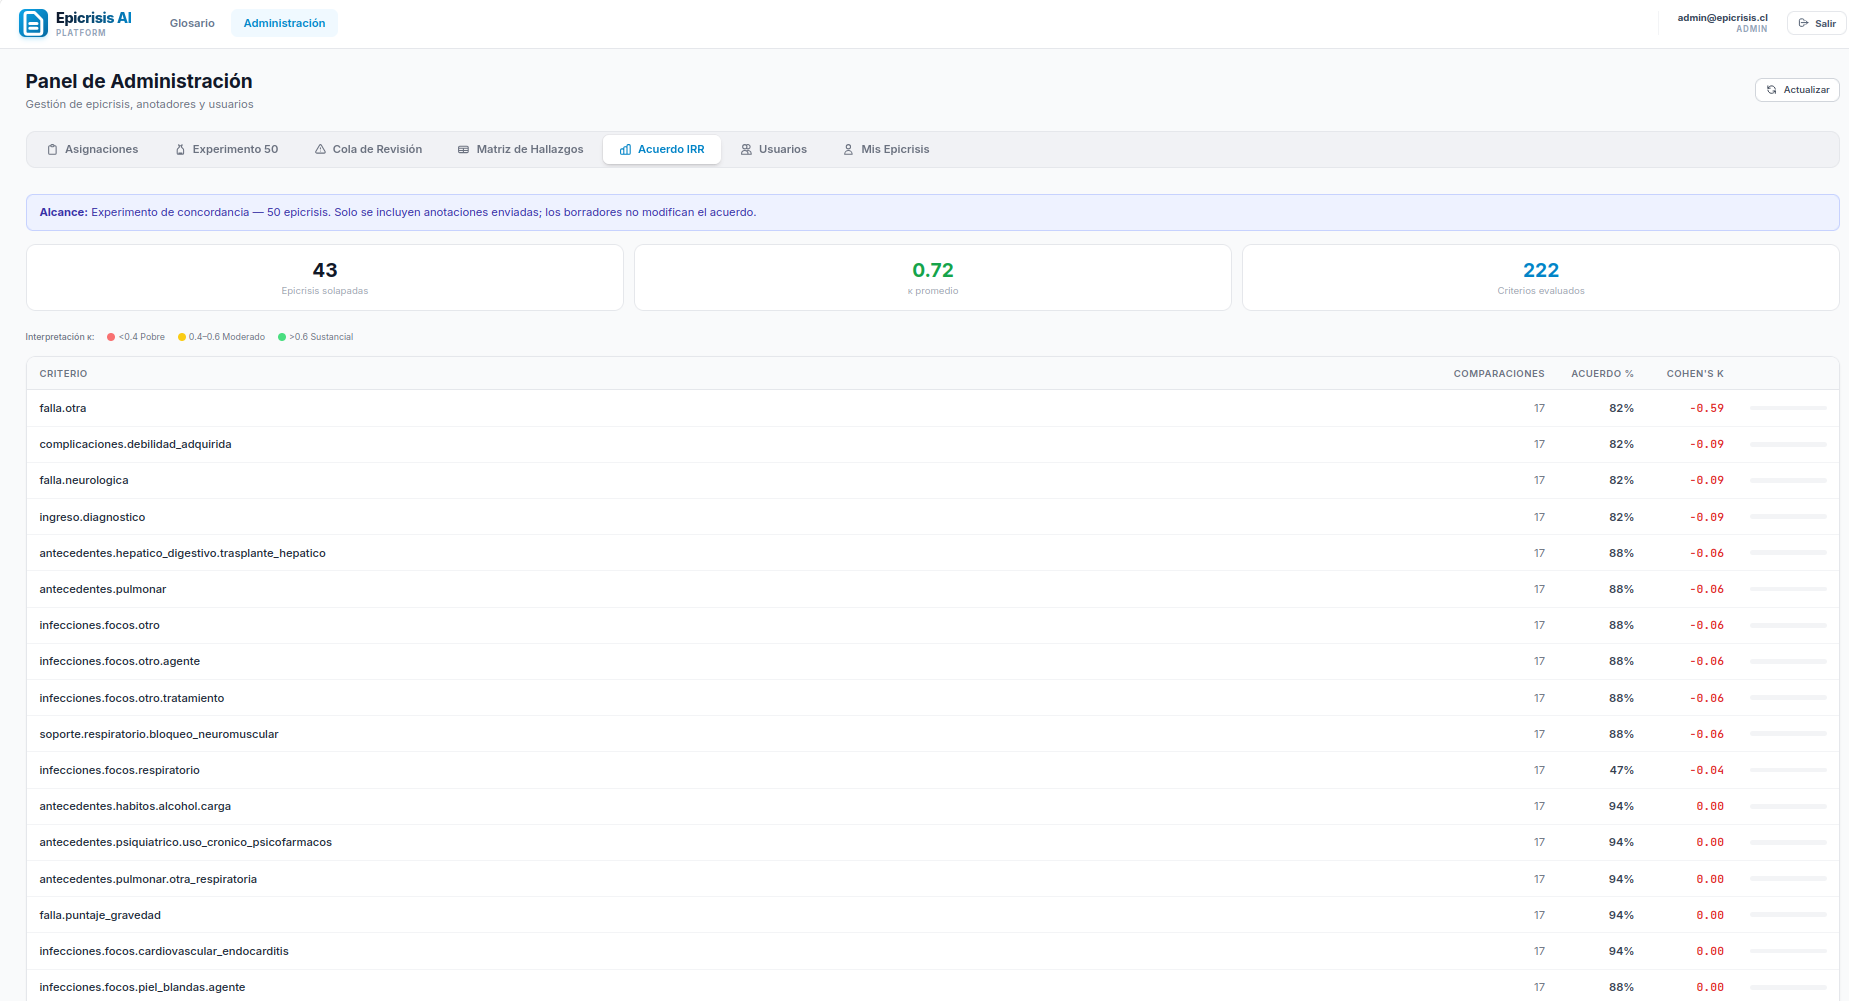
\includegraphics[width=0.95\textwidth]{figuras/capturas/panel_de_acuerdo.png}
\caption{Vista de acuerdo inter-anotador del panel de administración, al corte del 15 de septiembre de 2026: 43 epicrisis solapadas, kappa de Cohen promedio de 0,72 y 222 criterios evaluados, con el detalle por criterio ordenado desde los valores más bajos.}
\label{fig:irr}
\end{figure}

\subsection{Infraestructura confiable}

La plataforma opera con una base de datos PostgreSQL replicada cada hora hacia un proveedor secundario con verificación de conteos y alertas de frescura, y con una migración validada hacia un servicio administrado en la nube (región sudamericana) con conexión cifrada verificada, disponible como entorno de despliegue. La disponibilidad se vigila desde fuera de la infraestructura propia cada quince minutos. El incidente de exposición de datos de mayo y el respaldo silencioso de agosto fueron detectados, diagnosticados y resueltos, y ambos dejaron mecanismos permanentes de prevención. El desarrollo quedó respaldado por 47 historias de usuario, 7 registros de decisiones de arquitectura y una suite de más de 180 pruebas automatizadas entre frontend, backend y extremo a extremo.

\subsection{Discusión de la estrategia de extracción}

La elección entre una consulta única y varias consultas no tiene una respuesta obvia. La consulta única tiene a la vista todo el formulario y puede mantener la coherencia entre bloques, pero paga esa ventaja con salidas largas, más expuestas a truncamiento y a errores en las variables del final del formulario, y con un costo alto ante cualquier error, porque corregirlo exige regenerar las 199 variables. El \textit{harness} acorta cada salida, valida y reintenta solo el grupo que falla y permite procesar las llamadas en lote, pero cada grupo reconstruye el episodio clínico por su cuenta. El piloto mostró las dos caras: la consulta única también tuvo un error de relación jerárquica en su primer intento, de modo que tener todo a la vista no garantiza la coherencia, y el \textit{harness} falló justamente en una relación entre grupos.

La estrategia C busca conservar las ventajas de la división y devolver a cada grupo una lectura común del caso. Retoma el mapa inicial del caso que ya usaba el procedimiento exploratorio, ahora como una representación validada en la que cada afirmación cita la epicrisis. La idea tiene antecedentes. En epicrisis psiquiátricas, una extracción en dos etapas, primero eventos y tiempos y después rasgos del curso clínico, superó a la extracción directa en la variable más inferencial (Chen et al., 2026); en registros de cáncer, un sistema de varios agentes mejoró las variables que dependen del contexto, pero no las más estructuradas (Aal Abdulsalam et al., 2026). Fuera de la medicina, las arquitecturas de pizarra (\textit{blackboard}) coordinan especialistas independientes mediante una estructura de datos compartida (Erman et al., 1980), y \textit{Skeleton-of-Thought} genera primero un esquema de la respuesta y luego desarrolla sus partes en paralelo (Ning et al., 2024), el mismo patrón de cómputo de la estrategia C. En la búsqueda realizada no se encontró una comparación pareada de las tres estrategias sobre los mismos pacientes, el mismo formulario y el mismo modelo, y ese es el aporte metodológico de esta parte del trabajo.

Los antecedentes y el propio experimento de concordancia indican dónde buscar el efecto. Los criterios con menor acuerdo entre anotadores, como la identificación del foco respiratorio de infección (47\% de acuerdo), exigen integrar información dispersa a lo largo de la epicrisis, y son los mismos en que un modelo del caso compartido debería ayudar más. Por eso el análisis se estratificará por bloque del formulario y por la calidad de la nota (secciones vacías, estadía en UCI documentada), en lugar de reportar solo un promedio global.

La estrategia C tiene un riesgo propio: un error en el modelo del caso llega a las 18 llamadas. Para acotarlo, la epicrisis prevalece en cualquier conflicto, la evidencia debe citar la nota y un clínico auditará una muestra de modelos del caso para medir su exactitud y la propagación de sus errores. El diseño tiene además límites que se declaran: la estrategia C y las medidas de coherencia se agregaron después del piloto, aunque antes de cualquier comparación con la referencia humana; los modelos corren cuantizados a 4 bits por la memoria disponible en el clúster; la cohorte proviene de un solo hospital; y la referencia humana todavía no tiene un procedimiento de resolución de desacuerdos.

% ==================== IV. COMPETENCIAS ====================
\section{Competencias de perfil de egreso}

A lo largo del proyecto se evidenciaron de manera concreta las tres competencias del perfil de egreso declaradas en la inscripción, no solo en el resultado final, sino en el proceso: en las decisiones de arquitectura, en el trato con datos sensibles, en la evaluación experimental de tecnologías nuevas y en la operación de un sistema del que dependía el trabajo de un equipo clínico.

\subsection*{Desarrollar soluciones innovadoras basadas en conocimientos avanzados de Ingeniería de Computación}

La plataforma de anotación no es la aplicación de una receta conocida, sino una solución diseñada desde cero para un problema con restricciones poco habituales: los usuarios son profesionales clínicos sin formación técnica, los datos son sensibles al punto de que el archivo original no puede llegar al navegador, y el producto del sistema (el conjunto de referencia) debe ser defendible metodológicamente.

Esas restricciones exigieron decisiones de ingeniería no triviales. El visor seguro reconstruye cada página del documento a partir de su estructura visual almacenada en la base de datos, en lugar de servir el PDF, lo que permite anonimizar al vuelo y controlar exactamente qué información llega a cada rol. El formulario jerárquico traduce un árbol de 199 variables clínicas, con estados de duda, propagación entre variables dependientes y candados de protección, a un modelo de datos plano y consultable. La anonimización opera en memoria al momento de entrega, preservando los registros originales para el equipo investigador, y usa reemplazos de longitud equivalente para no descuadrar el posicionamiento absoluto del documento. Cada una de estas piezas aplica conocimientos de arquitectura de software, bases de datos, seguridad y diseño de sistemas interactivos a un problema abierto, y el conjunto forma un sistema que no existía en la organización y que hoy sostiene su línea de investigación clínica.

La extracción automática exigió decisiones del mismo tipo. Tras la validación del \textit{harness}, el modelo dejó de escribir la cita y pasó a indicar las líneas numeradas que respaldan cada valor, cuyo texto copia el programa, de modo que no puede inventar citas. En la comparación, las tres estrategias comparten esa forma de citar y un único validador, para que sus diferencias no provengan de cómo se revisan las respuestas, y en la estrategia C las 18 llamadas reciben un modelo del caso validado que no reemplaza a la epicrisis como fuente de la evidencia.

\subsection*{Aplicar diversos métodos de análisis de datos para la comprensión de los fenómenos abordados}

El análisis de datos atraviesa el proyecto de principio a fin. En la etapa exploratoria, el agrupamiento de comorbilidades sobre las primeras 27 epicrisis permitió identificar perfiles de paciente y dimensionar la viabilidad de la extracción estructurada.

En la evaluación de modelos, el contraste entre las corridas exploratorias y la validación del \textit{harness} mostró que su ventaja no podía atribuirse solo a la división del formulario, porque habían cambiado varias condiciones a la vez: con la misma detención de la generación, la consulta única de Gemma también dejó de truncarse. Para aislar el efecto de la división se diseñó un experimento controlado y pareado, con los tres modelos sobre una cohorte fija (las 50 epicrisis que revisan los anotadores) y con la consulta única frente al \textit{harness} como comparación principal, definida antes de contrastar cualquier salida con la referencia humana. En el piloto, la lectura de los errores identificó una falla entre grupos de variables que invalidó el caso aunque sus 199 variables tenían respuesta válida; esa falla motivó una tercera estrategia, el \textit{harness} con un modelo del caso compartido, sin alterar la comparación principal.

El experimento de concordancia entre anotadores es la aplicación más formal de esta competencia: mide la confiabilidad del conjunto de referencia mediante acuerdo entre evaluadores independientes, con selección determinista y reproducible de los 50 casos, tres revisores por caso y el cálculo de concordancia integrado al panel de administración. Este diseño reconoce algo que es fácil pasar por alto: antes de evaluar si una máquina extrae bien, hay que medir cuánto acuerdan los humanos entre sí, porque ese acuerdo es la cota superior de lo que tiene sentido exigirle al modelo. Como esa cota varía entre criterios, la concordancia se analizó por criterio y no solo en promedio, lo que permitió distinguir entre la paradoja del kappa y el desacuerdo genuino; con la misma lógica, la comparación de estrategias se estratificará por bloque del formulario y por calidad de la nota.

\subsection*{Investigar sobre nuevas tecnologías de información existentes en la industria y facilitar su adopción dentro de las organizaciones}

El proyecto exigió investigar tecnología que ni el estudiante ni la organización dominaban al inicio, y dejarla operativa para otros. El estudiante completó un programa de formación en aprendizaje profundo y modelos de lenguaje, aplicado en la evaluación de Gemma, Llama-70B y Qwen sobre el clúster ih-condor, que requirió resolver problemas concretos de adopción: la reserva de varias tarjetas gráficas para los modelos grandes y un procedimiento de instalación documentado para el equipo, porque los nodos del clúster no alcanzan el repositorio público de paquetes.

La comparación de estrategias exigió investigar más a fondo. La consulta única de Gemma no cabía en memoria (sin leer la entrada por trozos intentaba reservar 211~GiB), y hubo que sortear un defecto de la biblioteca de inferencia en el manejo de la caché, sin modificar la biblioteca y sin alterar la salida. El diseño de la estrategia C, a su vez, se contrastó con antecedentes de extracción por etapas y por varios agentes en registros clínicos (Chen et al., 2026; Aal Abdulsalam et al., 2026).

La dimensión de adopción organizacional es explícita en varios entregables: el manual de anotación interactivo dentro de la propia aplicación, que convierte el protocolo de anotación en ejercicios prácticos; el glosario clínico indexado por campo; la documentación del entorno de cómputo y la norma de ejecutar todo trabajo mediante el planificador de tareas del clúster; y el traslado de la base de datos, que tras el incidente de agosto pasó de una máquina personal a una estación de trabajo dedicada, con respaldo horario verificado hacia el servicio en la nube al que se validó su migración. Investigar tecnología nueva es la mitad de la competencia; la otra mitad es dejarla usable por otros.

En síntesis, las tres competencias operaron como momentos de un mismo ciclo: diseñar una solución, analizar lo que produce y dejarla operativa para el equipo. En la plataforma, el visor y la anonimización al vuelo permiten construir un conjunto de referencia cuya calidad mide el experimento de concordancia, todavía en ejecución, y el manual interactivo y la nueva infraestructura mantienen la plataforma en uso. En la extracción, el ciclo se recorrió varias veces: los límites de la consulta única con Gemma llevaron al \textit{harness}, el análisis de su ventaja condujo a la comparación controlada y la falla del piloto dio origen a la estrategia C. La corrida definitiva de esa comparación sigue pendiente.

% ==================== V. CONCLUSIONES ====================
\section{Conclusiones}

Este trabajo de título partió de un problema clínico real y terminó con un sistema en producción que lo ataca por su base: sin datos estructurados confiables no hay estadística, ni auditoría, ni predicción posible sobre los pacientes de una UCI. La plataforma de anotación construida, con su visor seguro, su formulario jerárquico y su experimento de concordancia, convierte el texto libre de las epicrisis en un conjunto de referencia con calidad medible. La evaluación de modelos de lenguaje abiertos sobre el clúster de iHealth, que avanzó desde una consulta única frágil hasta el diseño de una comparación controlada de tres estrategias de extracción, estableció además un marco reproducible para responder, una vez completada la corrida definitiva, la pregunta que sigue: cuánto de ese trabajo de anotación puede automatizarse sin sacrificar validez clínica, y con qué forma de consultar al modelo.

El proyecto también dejó aprendizajes que exceden lo técnico. Trabajar con datos de pacientes reales enseñó que la protección de datos no es una casilla de cumplimiento sino una práctica continua, que se endurece con cada caso límite descubierto. Operar un sistema del que depende un equipo enseñó que la confiabilidad se construye con verificación y monitoreo, no con optimismo: los dos incidentes del período (la sobreescritura de la base y el respaldo silencioso) fueron resueltos y convertidos en mecanismos permanentes de prevención. Y construir para usuarios clínicos enseñó que la adopción de tecnología es un problema de ingeniería por derecho propio, que se resuelve con manuales interactivos, glosarios y fricción cuidadosamente eliminada, no con capacitaciones de una vez.

\subsection{Trabajo futuro}

El trabajo deja abiertas líneas concretas, en orden de prioridad:

\begin{enumerate}
    \item \textbf{Cerrar la referencia humana.} Fijar el corte final del experimento de concordancia, definir cómo se resuelven los desacuerdos entre anotadores y recalcular la concordancia sobre la versión definitiva.
    \item \textbf{Ejecutar la comparación completa.} Correr las tres estrategias con los tres modelos sobre las 50 epicrisis, con un motor de inferencia que procese en lote las llamadas de cada caso, y reportar acuerdo, validez, evidencia, costo y coherencia clínica por estrategia, por bloque del formulario y por calidad de la nota.
    \item \textbf{Validar con el equipo clínico.} Acordar las reglas de coherencia entre bloques y el criterio de estadía en UCI documentada, y auditar una muestra de modelos del caso y del soporte de la evidencia citada sin que el revisor sepa qué estrategia la produjo.
    \item \textbf{Publicar el protocolo.} Se prepara un manuscrito que reporta la comparación de las tres estrategias con su plan de análisis preespecificado, para que otros equipos puedan replicarla con sus propios formularios.
    \item \textbf{Escalar y proyectar.} Extender la estrategia que resulte mejor a las 275 epicrisis y avanzar hacia los modelos predictivos de eventos clínicos que motivaron el proyecto desde su origen.
\end{enumerate}

La infraestructura, los datos y el marco de evaluación para ese camino quedaron construidos.

% ==================== BIBLIOGRAFÍA ====================
\newpage
\section*{BIBLIOGRAFÍA}
\addcontentsline{toc}{section}{BIBLIOGRAFÍA}

\begin{itemize}[leftmargin=1.27cm, label={}]
    \item Aal Abdulsalam, A., Al Zaabi, A., Jeeballah, R., \& El Keraby, H. (2026). A multi-agent open-source LLM for structured cancer registry information extraction from pathology and medical reports. En \textit{Proceedings of the 25th Workshop on Biomedical Language Processing (BioNLP 2026)} (pp. 531--551). Association for Computational Linguistics.
    \item Chen, C.-H., Tseng, P.-C., Dai, H.-J., Su, C.-H., Wang, S.-H., Chien, Y.-L., Huang, W.-L., Wu, C.-S., \& Chen, H.-H. (2026). Two-stage extraction of clinical course information from psychiatric discharge summaries using fine-tuned large language models: Cross-validation study. \textit{JMIR Formative Research, 10}, e94454.
    \item Erman, L. D., Hayes-Roth, F., Lesser, V. R., \& Reddy, D. R. (1980). The Hearsay-II speech-understanding system: Integrating knowledge to resolve uncertainty. \textit{ACM Computing Surveys, 12}(2), 213--253.
    \item Grattafiori, A., et al. (2024). \textit{The Llama 3 herd of models}. arXiv preprint arXiv:2407.21783.
    \item Landis, J. R., \& Koch, G. G. (1977). The measurement of observer agreement for categorical data. \textit{Biometrics, 33}(1), 159--174.
    \item Ning, X., Lin, Z., Zhou, Z., Wang, Z., Yang, H., \& Wang, Y. (2024). Skeleton-of-Thought: Prompting LLMs for efficient parallel generation. En \textit{The Twelfth International Conference on Learning Representations (ICLR 2024)}.
    \item Vaswani, A., Shazeer, N., Parmar, N., Uszkoreit, J., Jones, L., Gomez, A. N., Kaiser, Ł., \& Polosukhin, I. (2017). Attention is all you need. \textit{Advances in Neural Information Processing Systems, 30}.
\end{itemize}

% ==================== ANEXOS ====================
\newpage
\begin{center}
{\large\bfseries A N E X O S}
\end{center}
\addcontentsline{toc}{section}{ANEXOS}
\newpage

\section*{Anexo A: Resumen de dedicación por bitácora}
\addcontentsline{toc}{section}{Anexo A: Resumen de dedicación por bitácora}

\begin{table}[h]
\centering
\begin{tabular}{c >{\raggedright\arraybackslash}p{9.5cm} r}
\toprule
\textbf{Bitácora} & \textbf{Foco principal} & \textbf{Horas} \\
\midrule
1 & Conceptualización y análisis exploratorio de epicrisis & 40 \\
2 & Diseño del experimento y gestión de incidente de producción & 42 \\
3 & Pipeline de ingesta, anonimización y estabilización & 45 \\
4 & Visor seguro, ocultamiento de datos y formulario jerárquico & 40 \\
5 & Validaciones, fechas clínicas, manual interactivo y clúster & 80 \\
6 & Evaluación de tres modelos LLM y extracción por dominios & 80 \\
7 & Anonimizador reconstruido, 275 epicrisis y panel de administración & 82 \\
8 & Experimento de concordancia, nube, respaldos y monitoreo & 84 \\
9 & Causa raíz del incidente de agosto, acompañamiento del experimento y cierre del informe & 80 \\
\midrule
\multicolumn{2}{l}{\textbf{Total}} & \textbf{573} \\
\bottomrule
\end{tabular}
\caption{Dedicación registrada en las bitácoras de SIDING.}
\end{table}

\section*{Anexo B: Arquitectura de la plataforma}
\addcontentsline{toc}{section}{Anexo B: Arquitectura de la plataforma}

La plataforma se compone de tres capas: una aplicación web de anotación, una API con base de datos relacional, y una infraestructura de operación y monitoreo. A ellas se suma, como rama paralela, el entorno de evaluación de modelos de lenguaje en el clúster ih-condor (Figuras~\ref{fig:arquitectura} y~\ref{fig:monitoreo}).

El frontend es una aplicación de página única construida con Vue~3, TypeScript y Pinia, servida como sitio estático desde una CDN con despliegue automático en cada integración a la rama principal. Ofrece siete vistas principales: inicio de sesión, aceptación de consentimiento, panel del anotador, vista de anotación, guía interactiva, glosario clínico y panel de administración. La vista de anotación presenta dos paneles: a la izquierda, el documento (texto seccionado o layout posicional reconstruido desde el PDF); a la derecha, el formulario clínico definido como un árbol de 222 nodos con 199 variables hoja (174 booleanas ternarias, 11 fechas, 5 selectores y 9 de texto libre), con sinónimos y pistas de la clasificación internacional de enfermedades por variable. Componentes dedicados miden el tiempo activo de anotación, dificultan la captura de pantalla y validan el formulario antes del envío.

El backend es una API en Node con TypeScript, supervisada por un administrador de procesos en una estación de trabajo dedicada y expuesta a internet mediante un túnel SSH reverso hacia un servidor con pasarela HTTPS. La autenticación usa tokens firmados con expiración, contraseñas cifradas y dos roles (administrador y anotador) verificados en el servidor en cada petición: un anotador solo accede a las epicrisis que tiene asignadas. Un bloqueo cooperativo con expiración evita colisiones entre anotadores concurrentes; el envío de anotaciones corre en una transacción; y los casos con criterios no determinables sobre un umbral se derivan a revisión experta.

La base de datos es PostgreSQL, accedido mediante un ORM. El proyecto validó su migración a un servicio administrado en la nube (región sudamericana) con TLS verificado contra las autoridades certificadoras oficiales del proveedor; durante la ejecución del experimento de concordancia la base opera localmente, replicada cada hora hacia un proveedor secundario con verificación tabla por tabla. El esquema almacena las 275 epicrisis anonimizadas con su documento, el texto seccionado, el layout posicional, las anotaciones por usuario y criterio con su evidencia, las asignaciones y las cohortes de experimentos.

Una capa de anonimización en el servidor actúa como defensa en profundidad: además de la anonimización en origen (identificadores con hash criptográfico y mapeo cifrado fuera del repositorio), un módulo de redacción extrae del propio documento nombres, RUT, firmas médicas, teléfonos y direcciones, y los enmascara al vuelo en toda respuesta de la API, protegiendo más de 60 términos médicos contra falsos positivos. El navegador nunca recibe información identificatoria.

La operación se monitorea en lazos concéntricos: el supervisor de procesos reinicia servicios caídos en segundos; un bot de Telegram en proceso independiente emite cuatro reportes diarios de salud (API, túnel, frontend, base de datos y almacenamiento) y permite reiniciar la API remotamente; una verificación externa cada quince minutos ejercita el sistema desde fuera de la infraestructura propia; y un respaldo horario verificado por conteo tabla por tabla replica la base hacia un proveedor secundario, con volcados cifrados adicionales verificados por suma de comprobación.

\begin{figure}[htbp]
\centering
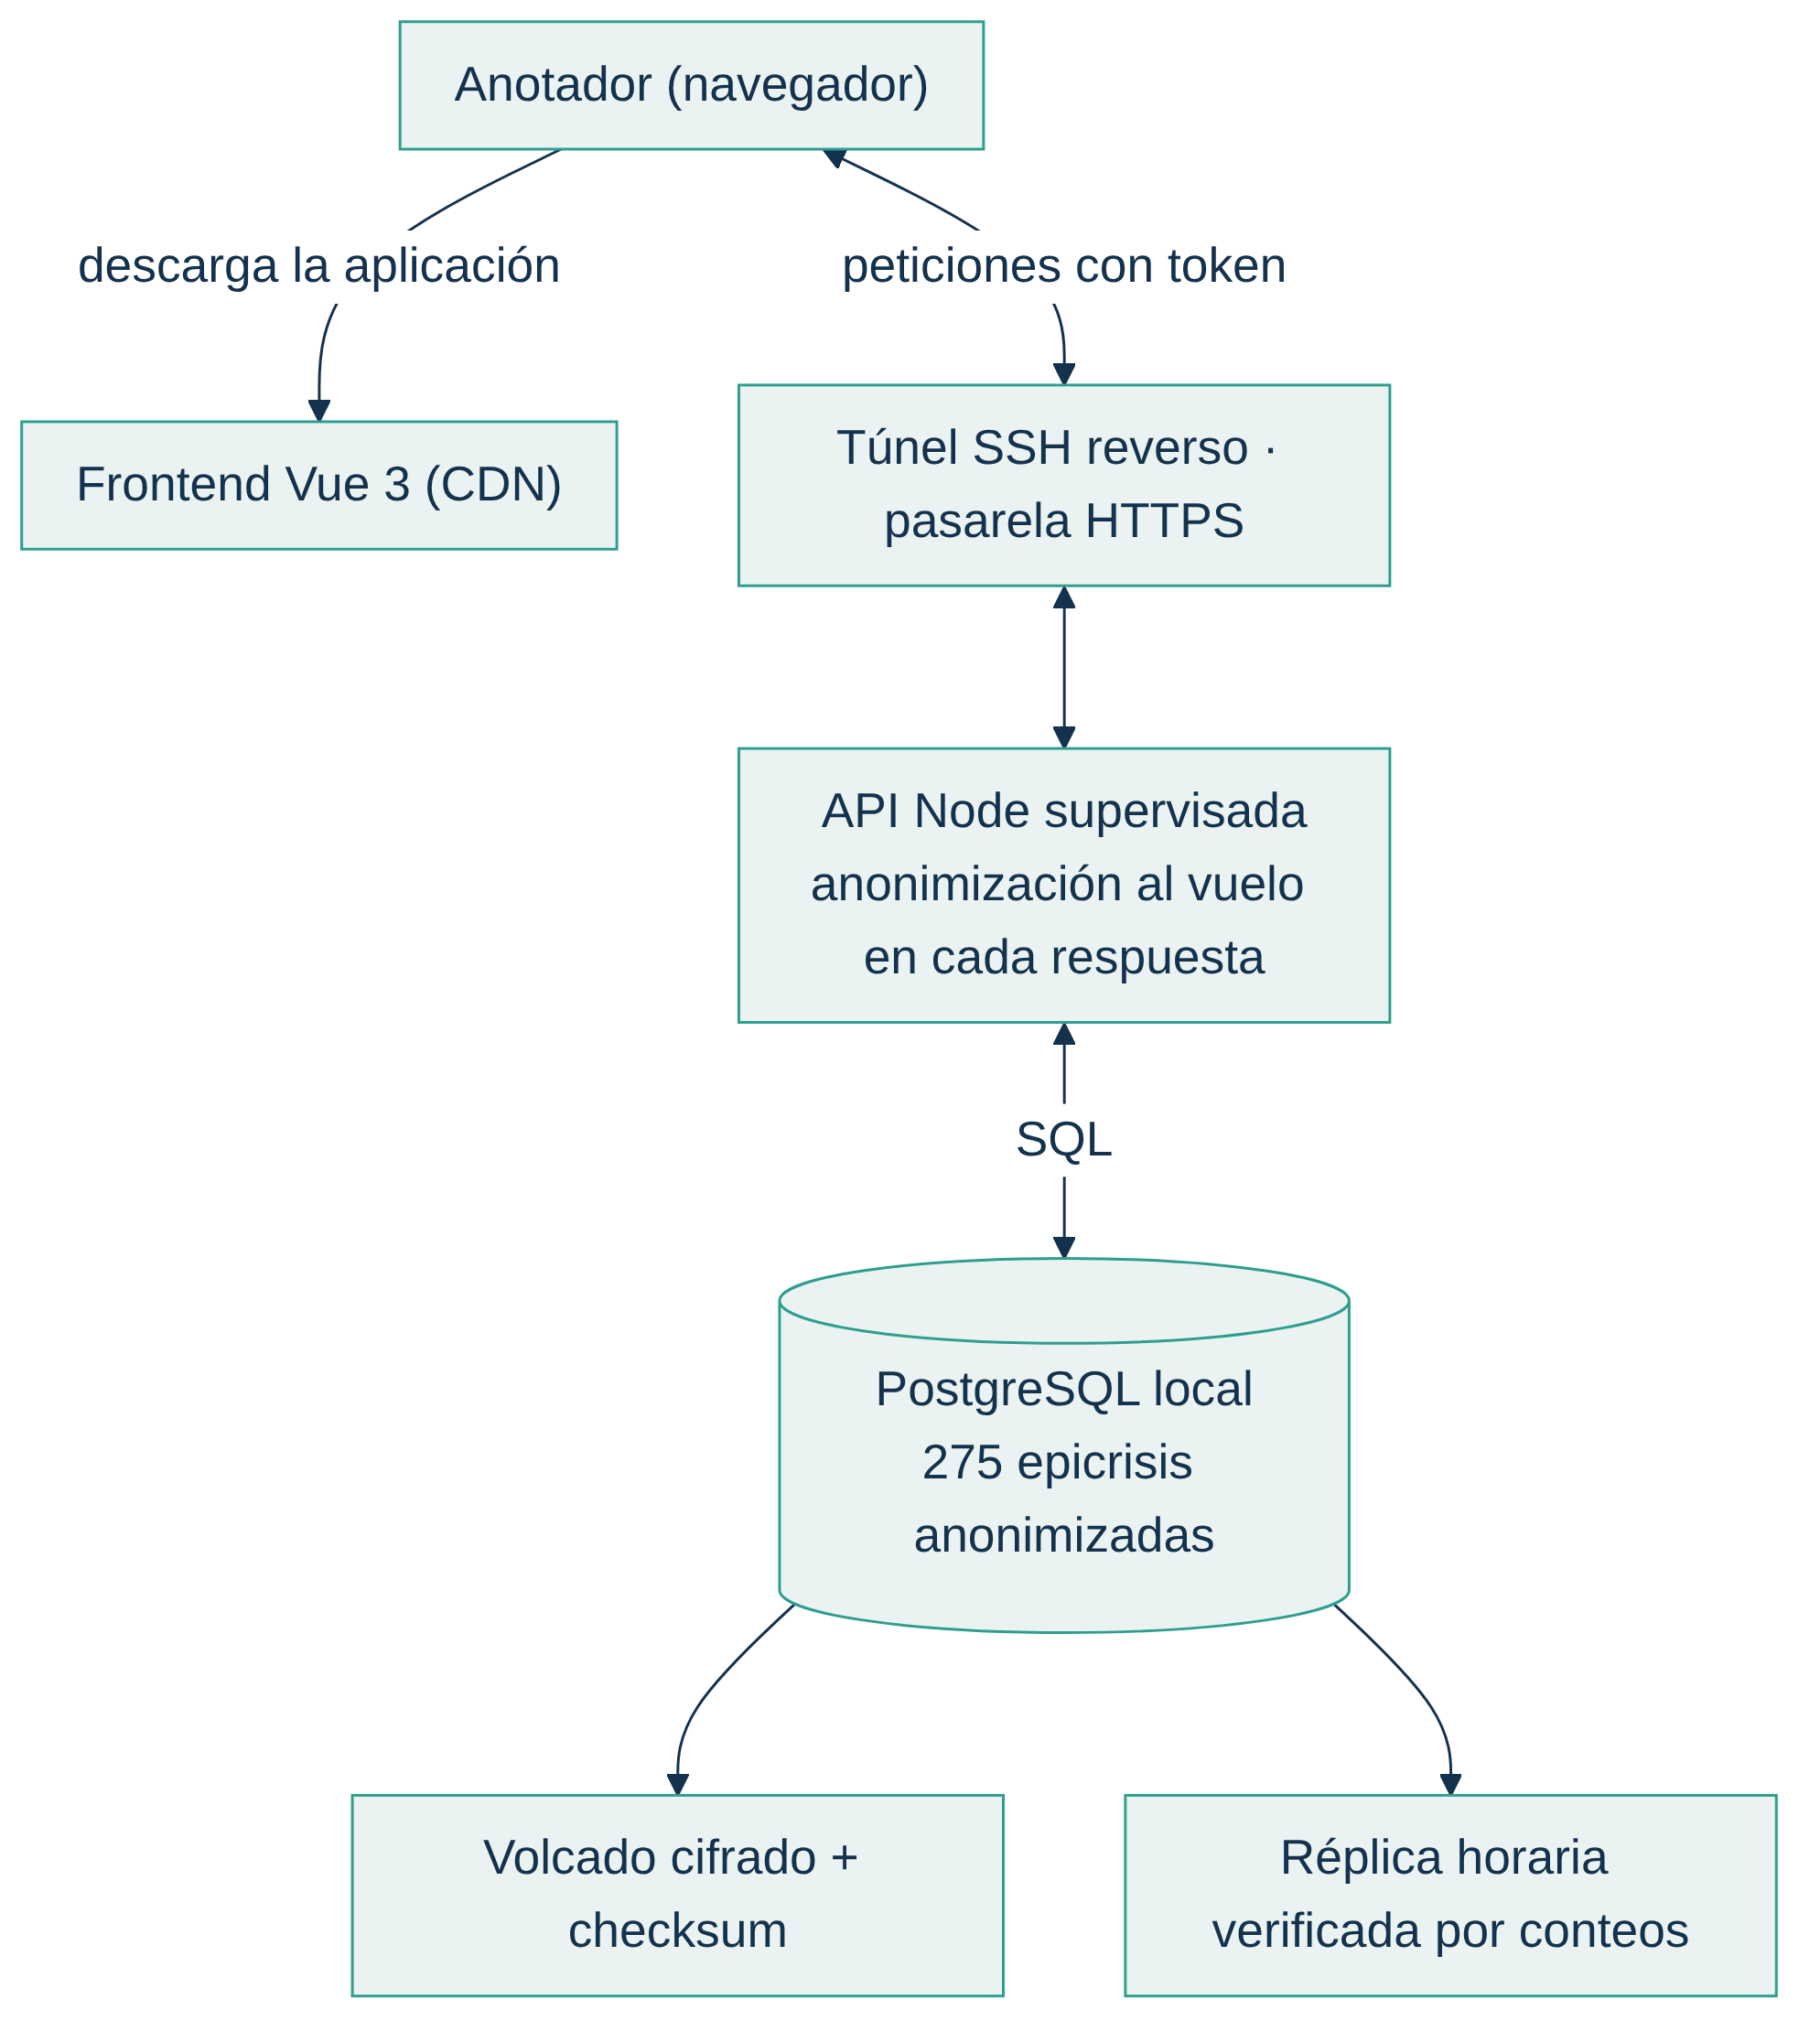
\includegraphics[width=0.78\textwidth]{figuras/diagramas/fig_plataforma.png}
\caption{Flujo de la plataforma de anotación: el anotador recibe la aplicación desde la CDN y conversa con la API a través del túnel HTTPS; la API anonimiza al vuelo cada respuesta y la base local se respalda por dos vías verificadas.}
\label{fig:arquitectura}
\end{figure}

\begin{figure}[htbp]
\centering
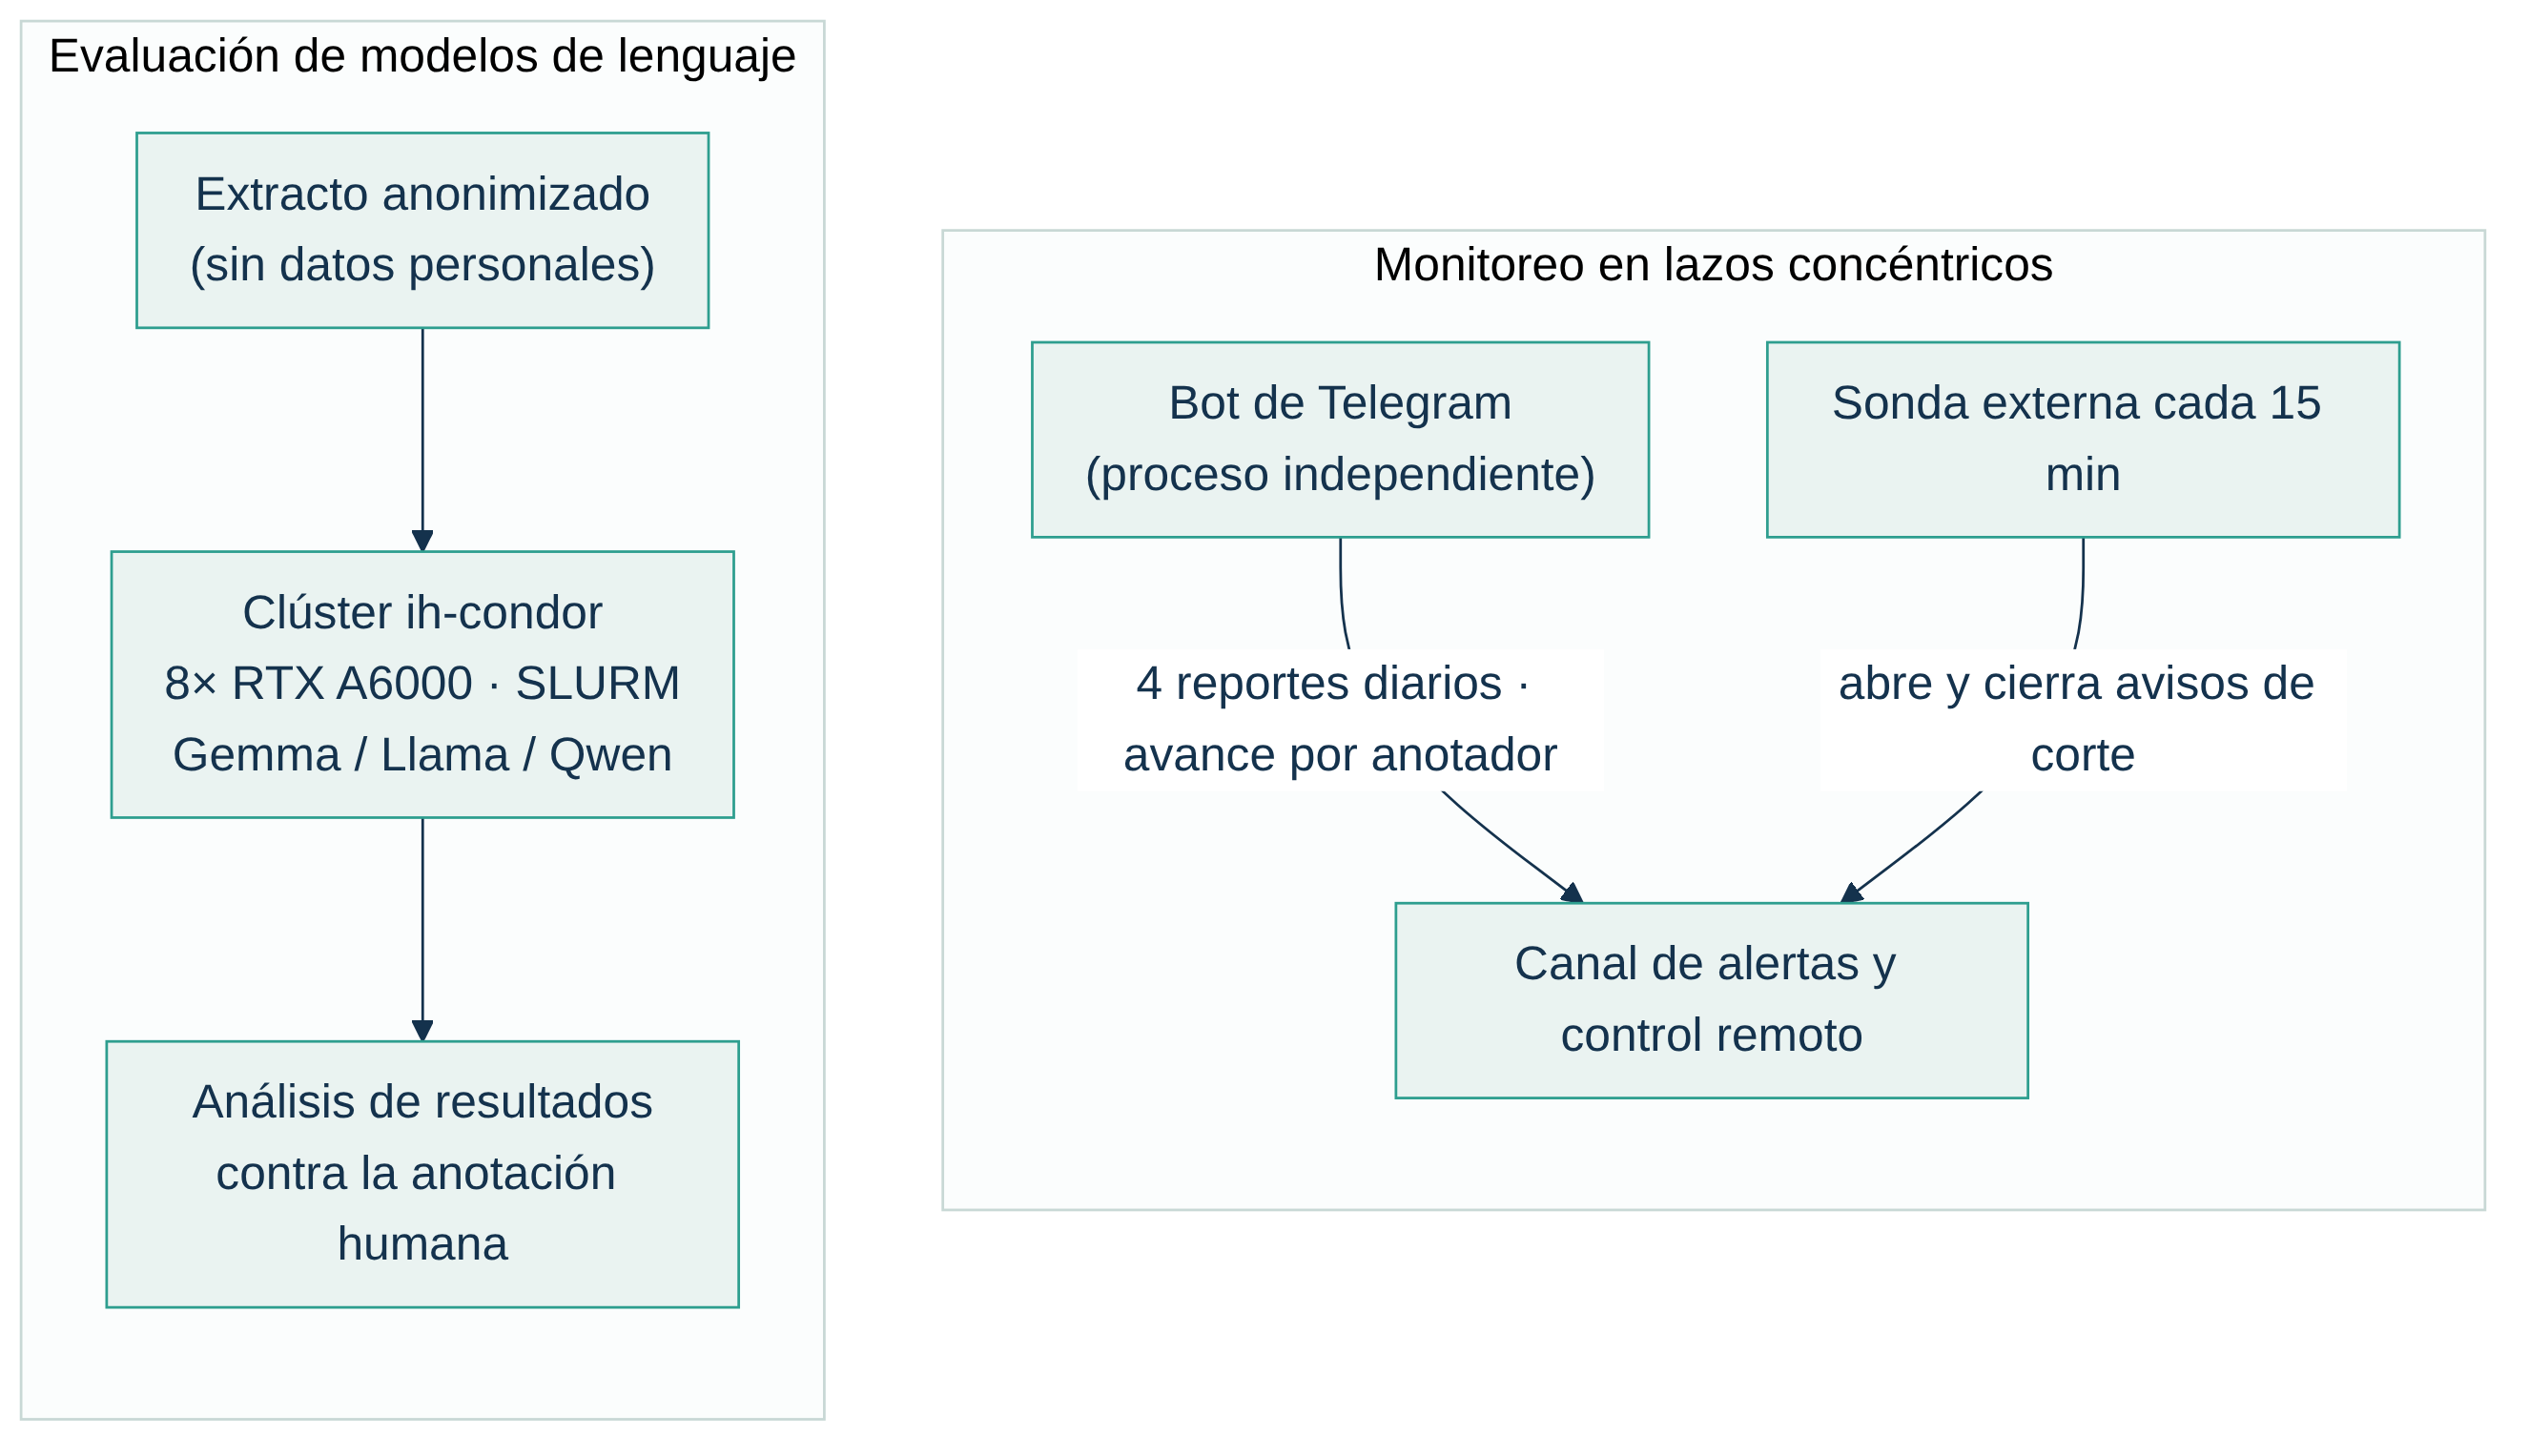
\includegraphics[width=0.95\textwidth]{figuras/diagramas/fig_monitoreo_cluster.png}
\caption{Monitoreo en lazos concéntricos (derecha) y evaluación de modelos de lenguaje en el clúster ih-condor (izquierda), alimentada solo con el texto anonimizado de las epicrisis; sus resultados se contrastarán con la anotación humana.}
\label{fig:monitoreo}
\end{figure}

\end{document}
